\newpage
\section{Pseudocode of Agentic Predictor} 
We present the pseudocode of the proposed \ours{} framework in \autoref{alg:pseudo_code} below.

\renewcommand{\algorithmiccomment}[1]{\textcolor{gray}{$\triangleright$ #1}}
\renewcommand{\algorithmicrequire}{\textbf{Initialization:}}
\renewcommand{\algorithmicensure}{\textbf{Input:}}

\begin{algorithm}[hbt]
\caption{Overall Procedure of \ours{}} \label{alg:pseudo_code}
\begin{algorithmic}[1]
\Require Multi-View Encoder $\mathrm{Enc(\cdot)}$ and Performance Predictor Model $\mathcal{M}_{\Theta}$
\Ensure User Instruction (or Task Description) $T \in \mathcal{T}$ and Training Data $D^{\text{train}}$

\State \Comment{Multi-View Graph Construction (\S\ref{section:multiview_encoding})}
\State Construct a node-aligned view set $\mathcal{G} = \{\mathcal{G}_v =(\mathcal{V}, \mathcal{E}, X_v )~\vert~ v\in \{\text{prompt}, \text{code}, \text{operator}\}\}$ where $X_v$ is the view-specific node features.
\State \Comment{Cross-Domain Unsupervised Pretraining (\S\ref{section:pretraining}, \emph{Optional})}
\State Sample $M$ unlabeled workflows $\mathcal{W}_1, \mathcal{W}_2, ..., \mathcal{W}_M$ from multiple domains
\For{each $\mathcal{W}_i = (\mathcal{G}_i, \mathcal{C}_i, \mathcal{P}_i)$}
    \State $\mathbf{Z}_i \gets \mathrm{Enc}(\mathcal{G}_i, \mathcal{C}_i, \mathcal{P}_i)$ \hfill\Comment{Encode multiview graph, code, and prompts}
    \State $(\hat{\mathcal{G}}_i, \hat{\mathcal{C}}_i, \hat{\mathcal{P}}_i) \gets \mathrm{Dec}(\mathbf{Z}_i)$ \hfill\Comment{Decode reconstructions}
\EndFor
\State $\mathcal{L}_{enc} = \mathcal{L}_{rec} + \mathcal{L}_{con}$ \hfill\Comment{Minimize total pretraining loss}

\State \Comment{Training Performance Predictor (\S\ref{section:predictor_search})}
\State Obtain (small) labeled dataset $\{(\mathcal{W}_j, T_j, e_j)\}_{j=1}^N$ from $D^{\text{train}}$
\For{each $(\mathcal{W}_j, T_j)$}
    \State $\mathbf{Z}_j \gets \mathrm{Enc}(\mathcal{W}_j)$ \hfill\Comment{Encode workflow}
    \State $\mathbf{T}_j \gets \text{TaskEncoder}(T_j)$ \hfill\Comment{Encode task description}
    \State $\mathcal{F}_j \gets \mathrm{MLP}([\mathbf{Z}_j, \mathbf{T}_j])$ \hfill\Comment{Form joint representation}
    \State $\hat{e}_j \gets \mathcal{M}_{\Theta}(\mathcal{F}_j)$ \hfill\Comment{Predict performance}
\EndFor
\State Train $\mathcal{M}_{\Theta}$ using binary cross-entropy loss $\mathcal{L}_{pred}(e_j, \hat{e}_j)$, where $\{e_j\}_{j=1}^N$

\State \Comment{Predictor-Guided Candidate Ranking}
\State Sample $K$ candidate workflows $\{\mathcal{W}_k\}_{k=1}^K$
\For{each $\mathcal{W}_k$}
    \State $\mathbf{Z}_k \gets \mathrm{Enc}(\mathcal{W}_k)$ \hfill\Comment{Encode workflow}
    \State $\mathcal{F}_k \gets \mathrm{MLP}([\mathbf{Z}_k, \mathbf{T}])$ \hfill\Comment{Encode task}
    \State $\hat{e}_k \gets \mathcal{M}_{\Theta}(\mathcal{F}_k)$ \hfill\Comment{Predict score}
\EndFor
\State Rank all $\{\mathcal{W}_k\}$ by predicted scores $\hat{e}_k$
\State \Return top-$k$ ranked workflows for final evaluation


\end{algorithmic}
\end{algorithm}






\section{Additional Experimental Results} \label{section:extra_results}
This section provides complementary studies that further characterize our approach: robustness when the agent-controller LLM backbone varies (\S\ref{section:llm_backbone_results}); an ablation over multiple GNN backbones (\S\ref{section:gnn_backbone_reesults}); a comparison to few-shot LLM predictors (\S\ref{section:llm_fewshot_results}); and out-of-distribution (OOD) generalization evaluations (\S\ref{section:ood_results}).





\subsection{Performance on Different LLM Backbones} \label{section:llm_backbone_results}

As shown in \autoref{table:llm_backbones}, we assess whether predictor performance is robust when the agentic workflows are driven by different LLMs. Concretely, we replicate our evaluation while swapping the controller LLM among GPT-4o-mini, DeepSeek, Qwen 7B, and Mistral 7B, holding the training data construction, multi-view encoder, and evaluation protocol fixed. Except for the Mistral 7B case, \ours{} exhibits stable performance and preserves the relative ranking of workflows across these backbones, indicating that it captures structural and behavioral regularities of agentic programs rather than idiosyncrasies of any single LLM.

\subsection{Performance on Different GNN Backbones}  \label{section:gnn_backbone_reesults}
Our main experiments use a 2-layer GCN (hidden size 512) following the standard setup in FLORA-Bench\,\citep{FLORA_Bench_25}, enabling a controlled comparison to baseline predictors. To test architecture sensitivity, we conduct an ablation over five diverse GNN backbones---GCN, GAT, GCN-II, Graph Transformer, and Dir-GNN---while keeping the prompt and code views fixed. As presented in \autoref{table:gnn_backbones} All backbones yield comparable predictive accuracy and replicate the same trends, reinforcing that the performance improvements stem from the multi-view encoding and pretraining rather than a specific GNN design. These results support the architecture-agnostic nature of the Agentic Predictor.

\subsection{Comparison with LLM Predictors} \label{section:llm_fewshot_results}
We compare against few-shot, prompt-based LLM classifiers implemented with a standardized LLM-PP–style template\,\citep{LLM_PP} with 5-shot and temperature set to 0 using GPT-4.1, Claude 4 Sonnet, and Gemini 2.5 Flash. The results in \autoref{table:llm_fewshot_results} are consistent with prior findings on FLORA-Bench\,\citep{FLORA_Bench_25} (which evaluated DeepSeek-v3), these prompted LLMs underperform even a simple MLP predictor and substantially trail our graph-based approach. A likely reason is that prompted LLM classifiers do not exploit the structured execution patterns and tool-usage dynamics present in agentic workflows. Beyond accuracy, prompted LLM inference incurs a per-sample monetary and latency cost, whereas our predictor amortizes cost at training time. In our setup, generating predictions for up to 1,000 samples per task with LLM prompting required approximately \$300, implying considerably higher expense at full-benchmark scale. By contrast, the learned predictor scales to large candidate sets with constant per-sample computational cost at inference. Overall, while few-shot LLMs provide a useful baseline, they are less effective and less economical for large-scale agent search.

\subsection{Out-of-Distribution (OOD) Generalization Performance} \label{section:ood_results}
We study two factors that enable OOD robustness. First, the multi-view encoder jointly represents workflows via graph, code, and prompt views, all of which are architecture-agnostic. This design allows unseen agents and tools to be incorporated as long as their implementations and textual descriptions are available; the graph encoder embeds novel entities through structural and attribute signals without relying on fixed IDs. Second, cross-domain unsupervised pretraining over diverse unlabeled workflows equips the encoder with priors over common structural and behavioral motifs (e.g., tool invocation patterns and reasoning flows), improving robustness to unseen configurations.

Regarding evaluation, following RQ3 in FLORA-Bench~\citep{FLORA_Bench_25}, we perform two levels of OOD generalization. \emph{Cross-system generalization:} train on one agentic framework (e.g., AFlow\,\citep{AFlow_ICLR_25}) and test on another (e.g., G-Designer\,\citep{GDesigner_ICML_25}) as well as \emph{cross-domain generalization:} train on one set of downstream tasks (e.g., math) and test on disjoint tasks (e.g., coding) not observed during training. As presented in \autoref{table:ood_aflow}, \autoref{table:ood_gd} and \autoref{table:cross_domain}, across both settings, \ours{} maintains strong performance and preserves relative workflow rankings, indicating that it generalizes beyond in-distribution memorization. 




\begin{table}[t]
\centering
\caption{Results on different backbones driven agentic workflows.}
\label{table:llm_backbones}
\resizebox{0.8\textwidth}{!}{%
\begin{tabular}{@{}c|cc|cc|cc|cc@{}}
\toprule
\textbf{Domain} & \multicolumn{2}{c}{\textbf{GPT-4o-mini}} & \multicolumn{2}{|c}{\textbf{DeepSeek}} & \multicolumn{2}{|c}{\textbf{Qwen 7B}} & \multicolumn{2}{|c}{\textbf{Mistral 7B}} \\ \midrule
\textbf{Model} & \textbf{Accuracy} & \textbf{Utility} & \textbf{Accuracy} & \textbf{Utility} & \textbf{Accuracy} & \textbf{Utility} & \textbf{Accuracy} & \textbf{Utility} \\ \midrule \midrule
MLP & 83.88 & 76.16 & 85.89 & 71.72 & 84.25 & 80.52 & 89.23 & 85.07 \\
GCN & 82.94 & 80.40 & 86.56 & 75.69 & 86.71 & 84.48 & 92.58 & 88.48 \\
GAT & 83.03 & 80.25 & 84.42 & 75.18 & 86.98 & 84.26 & 92.62 & 88.72 \\
GCN-II & 82.81 & 79.48 & 84.34 & 75.68 & 85.17 & 82.71 & 90.94 & 85.89 \\
Graph Transformer & 83.42 & 79.83 & 86.34 & 73.06 & 86.76 & 84.65 & \textbf{92.80} & \textbf{88.87} \\
Dir-GNN & 84.85 & 79.81 & 85.38 & 71.27 & 86.36 & 84.50 & 91.87 & 88.47 \\
One For All & 81.24 & 71.92 & 84.73 & 73.23 & 84.51 & 80.42 & 89.13 & 85.06 \\ \midrule
\emph{\ours{}} & \textbf{85.33} & \textbf{81.42} & \textbf{88.39} & \textbf{76.64} & \textbf{86.99} & \textbf{85.02} & 92.33 & 88.69 \\ \bottomrule
\end{tabular}%
}
\end{table}



\begin{table}[t]
\centering
\caption{Results on different GNN backbones of \ours{}.} \label{table:gnn_backbones}
\resizebox{0.8\textwidth}{!}{%
\begin{tabular}{@{}c|cc|cc|cc|cc@{}}
\toprule
 \textbf{Domain} & \multicolumn{2}{c}{\textbf{Code Generation}} & \multicolumn{2}{|c}{\textbf{Math Problem}} & \multicolumn{2}{|c}{\textbf{Common Reasoning}} & \multicolumn{2}{|c}{\textbf{Average}} \\ \midrule
\textbf{GNN Backbone} & \textbf{Accuracy} & \textbf{Utility} & \textbf{Accuracy} & \textbf{Utility} & \textbf{Accuracy} & \textbf{Utility} & \textbf{Accuracy} & \textbf{Utility} \\ \midrule \midrule
GCN & 85.62 & 80.08 & 79.56 & 74.08 & 87.96 & 91.47 & 84.38 & 81.88 \\
GAT & 83.74 & 73.11 & 75.86 & 67.03 & 86.95 & 87.20 & 82.19 & 75.78 \\
GCN-II & 84.71 & 73.83 & 76.68 & 68.41 & 86.76 & 86.04 & 82.72 & 76.09 \\
Graph Transformer & 83.22 & 78.17 & 76.64 & 70.03 & 86.88 & 89.50 & 82.25 & 79.23 \\
Dir-GNN & 84.62 & 79.64 & 80.26 & 75.03 & 87.93 & 94.77 & 84.27 & 83.15 \\ \bottomrule
\end{tabular}%
}
\end{table}


\begin{table}[t]
\centering
\caption{Comparison between \ours{} and LLM-based few-show classification.} \label{table:llm_fewshot_results}
\resizebox{0.8\textwidth}{!}{%
\begin{tabular}{@{}c|cc|cc|cc|cc@{}}
\toprule
\textbf{Domain} & \multicolumn{2}{c}{\textbf{Code Generation}} & \multicolumn{2}{|c}{\textbf{Math Problem}} & \multicolumn{2}{|c}{\textbf{Common Reasoning}} & \multicolumn{2}{|c}{\textbf{Average}} \\ \midrule
\textbf{Model} & \textbf{Accuracy} & \textbf{Utility} & \textbf{Accuracy} & \textbf{Utility} & \textbf{Accuracy} & \textbf{Utility} & \textbf{Accuracy} & \textbf{Utility} \\ \midrule \midrule
GPT-4.1 ($\sim$\$59) & 62.42 & 57.00 & 67.08 & 52.97 & 59.10 & 66.79 & 62.86 & 58.92 \\
Claude 4 Sonnet ($\sim$\$202) & 56.72 & 51.65 & 64.62 & 57.32 & 44.50 & 41.25 & 55.28 & 50.07 \\
Gemini 2.5 Flash ($\sim$\$21) & 60.52 & 58.94 & 51.60 & 55.21 & 59.20 & 63.17 & 57.10 & 59.11 \\ \midrule
\emph{\ours{}} & \textbf{84.40} & \textbf{78.84} & \textbf{80.10} & \textbf{77.61} & \textbf{90.40} & \textbf{87.67} & \textbf{84.97} & \textbf{81.37} \\ \bottomrule
\end{tabular}%
}
\end{table}






\begin{table}[t]
\centering
\caption{Results when train on AFlow and test on G-Designer.}
\label{table:ood_aflow}
\resizebox{0.8\textwidth}{!}{%
\begin{tabular}{@{}c|cc|cc|cc|cc@{}}
\toprule
\textbf{Domain} & \multicolumn{2}{c}{\textbf{Code Generation}} & \multicolumn{2}{|c}{\textbf{Math Problem}} & \multicolumn{2}{|c}{\textbf{Common Reasoning}} & \multicolumn{2}{|c}{\textbf{Average}} \\ \midrule
\textbf{Model} & \textbf{Accuracy} & \textbf{Utility} & \textbf{Accuracy} & \textbf{Utility} & \textbf{Accuracy} & \textbf{Utility} & \textbf{Accuracy} & \textbf{Utility} \\ \midrule \midrule
GCN & 56.76 & 54.29 & 49.64 & 51.92 & 61.37 & 54.13 & 55.92 & 53.45 \\
GAT & 57.25 & 56.05 & 48.29 & 48.71 & 57.03 & 53.12 & 54.19 & 52.63 \\
GCN-II & 64.16 & 62.67 & 48.85 & 50.56 & 65.55 & 52.76 & 59.52 & 55.33 \\
Graph Transformer & 60.83 & 58.39 & 47.73 & 46.65 & 55.88 & 48.87 & 54.81 & 51.30 \\
One For All & 58.97 & 53.25 & 50.60 & 51.02 & 63.84 & 55.22 & 57.80 & 53.16 \\ \midrule
\emph{\ours{}} & \textbf{65.02} & \textbf{64.91} & \textbf{53.62} & \textbf{52.83} & \textbf{67.51} & \textbf{57.74} & \textbf{62.05} & \textbf{58.49} \\ \bottomrule
\end{tabular}%
}
\end{table}


\begin{table}[t]
\centering
\caption{Results when train on G-Designer and test on AFlow.}
\label{table:ood_gd}
\resizebox{0.8\textwidth}{!}{%
\begin{tabular}{@{}c|cc|cc|cc|cc@{}}
\toprule
\textbf{Domain} & \multicolumn{2}{c}{\textbf{Code Generation}} & \multicolumn{2}{|c}{\textbf{Math Problem}} & \multicolumn{2}{|c}{\textbf{Common Reasoning}} & \multicolumn{2}{|c}{\textbf{Average}} \\ \midrule
\textbf{Model} & \textbf{Accuracy} & \textbf{Utility} & \textbf{Accuracy} & \textbf{Utility} & \textbf{Accuracy} & \textbf{Utility} & \textbf{Accuracy} & \textbf{Utility} \\ \midrule \midrule
GCN & 58.21 & 57.33 & 67.57 & 54.63 & 57.51 & 53.37 & 61.10 & 55.11 \\
GAT & 59.29 & 59.68 & 66.34 & 52.70 & 56.07 & 50.38 & 60.57 & 54.25 \\
GCN-II & 58.75 & 61.17 & 67.32 & 52.96 & 55.93 & 52.19 & 60.67 & 55.44 \\
Graph Transformer & 60.52 & \textbf{61.44} & 58.97 & 57.49 & 56.50 & 54.86 & 58.66 & 57.93 \\
One For All & \textbf{62.01} & 54.57 & 58.72 & 61.23 & \textbf{59.40} & 54.17 & 60.04 & 56.66 \\ \midrule
\emph{\ours{}} & 60.94 & 59.75 & \textbf{69.11} & \textbf{63.02} & 58.56 & \textbf{56.73} & \textbf{62.87} & \textbf{59.83} \\ \bottomrule
\end{tabular}%
}
\end{table}


\begin{table}[t]
\centering
\caption{Results on cross-domain OOD test.}
\label{table:cross_domain}
\resizebox{\textwidth}{!}{%
\begin{tabular}{@{}c|cc|cc|cc|cc|cc|cc|cc@{}}
\toprule
\textbf{Domain} & \multicolumn{2}{c}{\textbf{Code-Math}} & \multicolumn{2}{|c}{\textbf{Code-Reason}} & \multicolumn{2}{|c}{\textbf{Math-Reason}} & \multicolumn{2}{|c}{\textbf{Math-Code}} & \multicolumn{2}{|c}{\textbf{Reason-Code}} & \multicolumn{2}{|c}{\textbf{Reason-Math}} & \multicolumn{2}{|c}{\textbf{Average}} \\ \midrule
\textbf{Model} & \textbf{Accuracy} & \textbf{Utility} & \textbf{Accuracy} & \textbf{Utility} & \textbf{Accuracy} & \textbf{Utility} & \textbf{Accuracy} & \textbf{Utility} & \textbf{Accuracy} & \textbf{Utility} & \textbf{Accuracy} & \textbf{Utility} & \textbf{Accuracy} & \textbf{Utility} \\ \midrule \midrule
GCN & 48.89 & 54.07 & 52.61 & 53.29 & 49.38 & 46.69 & 50.07 & 48.75 & 32.56 & 50.53 & 33.42 & 50.57 & 44.49 & 50.65 \\
GAT & 45.95 & 49.42 & 53.71 & 57.90 & 46.83 & 38.90 & 51.02 & 47.40 & 33.79 & 52.62 & 33.42 & 51.10 & 44.12 & 49.56 \\
GCN-II & 56.02 & 44.49 & 53.44 & 45.93 & 50.38 & 47.36 & 39.48 & 51.55 & 38.13 & 51.35 & 36.61 & \textbf{57.93} & 45.68 & 49.77 \\
Graph Transformer & 47.67 & 56.18 & 53.71 & 57.95 & 47.90 & 43.63 & 54.00 & 56.20 & 60.92 & 52.37 & 41.77 & 52.91 & 51.00 & 53.21 \\
One For All & 36.61 & \textbf{61.11} & 50.33 & 39.82 & 44.92 & 45.88 & \textbf{65.40} & 56.24 & \textbf{63.36} & 50.60 & 38.08 & 45.27 & 49.78 & 49.82 \\ \midrule
\textit{\ours{}} & \textbf{57.17} & 61.03 & \textbf{54.22} & \textbf{62.99} & \textbf{53.86} & \textbf{61.75} & 59.88 & \textbf{60.25} & 61.60 & \textbf{54.52} & \textbf{62.90} & 52.69 & \textbf{58.27} & \textbf{58.87} \\ \bottomrule
\end{tabular}%
}
\end{table}

\subsection{Effects of Pretraining Phase (Full Results)} \label{section:full_pretrain}
Since acquiring a large amount of ground-truth labels from agentic workflows is expensive, we examine whether cross-domain unsupervised pretraining (denoted as \ours{}+) benefits settings where labeled instances are limited. We vary the label ratio from 0.1 to 0.5, selecting labeled samples from the training split of all datasets in the benchmark. Concretely, we construct an unlabeled corpus by pooling all workflow configurations from the remaining training splits of the FLORA-Bench across Code, Math, and Reasoning tasks and both AFlow and G‑Designer frameworks, sampling uniformly over the pool without additional deduplication or domain re‑weighting. This yields $M = 232,104$ distinct samples ($\approx$ 6.56\% Code, 2.86\% Math, 90.58\% Reasoning). No validation and test workflows or labels are included to avoid leakage. We pretrain the proposed multi-view encoder with a batch size of 32 for 20 epochs. 

Following the average results in the main text, we provide a comprehensive comparison of accuracy (top row) and utility (bottom row) across three task domains---code generation, math problems, and reasoning---under varying label ratios from 0.5 to 0.1 (\autoref{figure:label_ratio_full_results}).

Across all settings, our proposed framework, \ours{}, and its pretrained variant, \ours{}+, consistently outperform baseline models, especially in low-resource scenarios. In the code generation domain (Figures~\ref{figure:label_ratio_coding_accuracy}, \ref{figure:label_ratio_coding_utility}), \ours{}+ achieves superior accuracy and notably higher utility as the label ratio decreases, outperforming all graph-based and non-graph baselines. Similarly, for math problems (Figures~\ref{figure:label_ratio_math_accuracy}, \ref{figure:label_ratio_math_utility}), \ours{}+ maintains a stable accuracy even as labeled data diminishes, while significantly improving utility, indicating better performance in label-scarce conditions. In reasoning tasks (Figures~\ref{figure:label_ratio_reason_accuracy}, \ref{figure:label_ratio_reason_utility}), although accuracy deltas narrow between models, \ours{}+ sustains strong utility across all label ratios, highlighting its robustness in generalization. When averaged across domains (Figures~\ref{figure:label_ratio_average_accuracy}, \ref{figure:label_ratio_average_utility}), \ours{}+ shows clear advantages in both metrics under limited supervision. The utility improvements are particularly prominent, suggesting that our pretrained encoder captures transferable representations that enhance decision-making, even when fine-tuning data is sparse. These findings validate the efficacy of the unsupervised pretraining phase and highlight the importance of cross-domain datasets for pretraining.


\begin{figure}[!t]
    \centering
    \subfloat[Code Generation.]{
        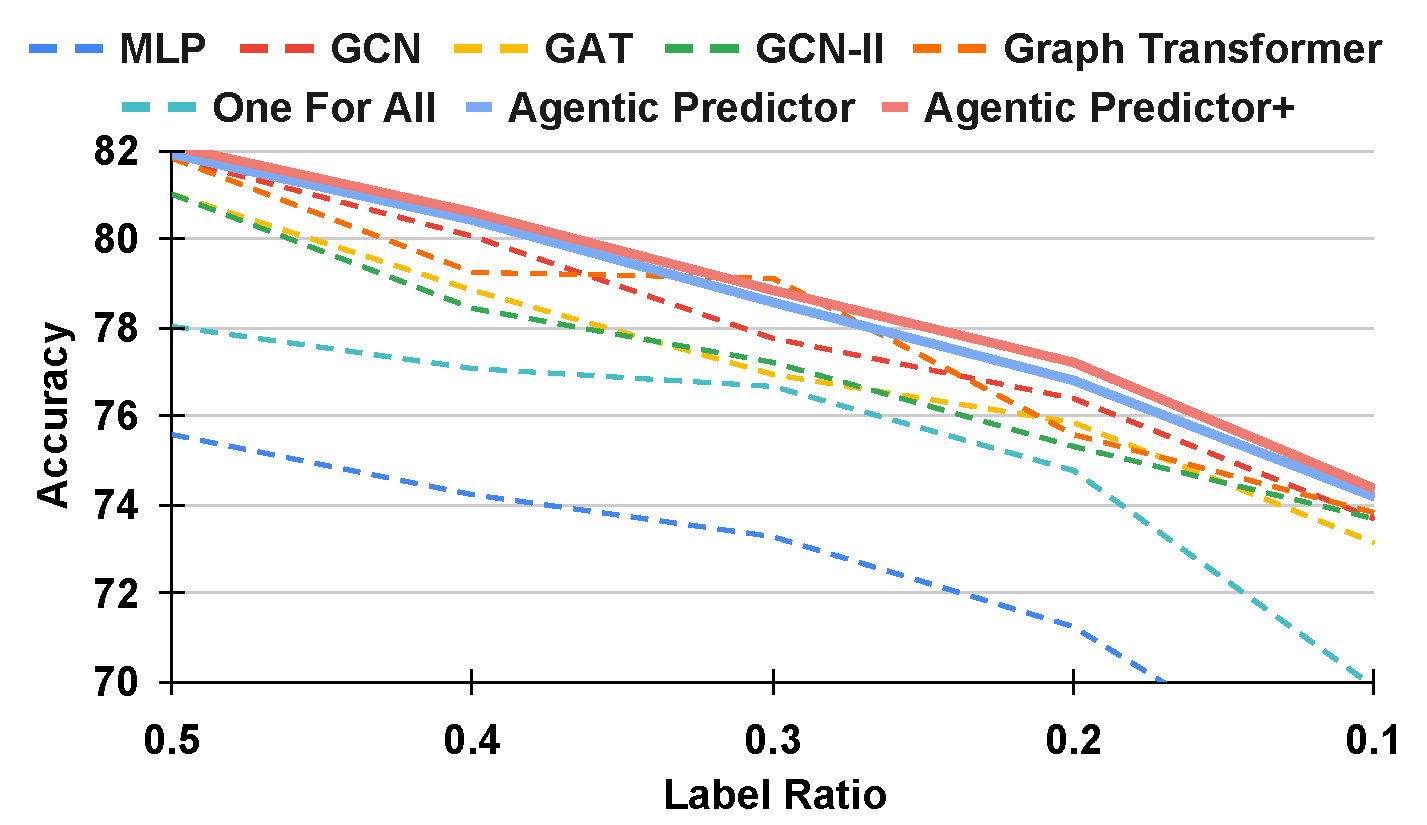
\includegraphics[width=0.24\textwidth]{figures/label_ratio_coding_acc.pdf}%
        \label{figure:label_ratio_coding_accuracy}
    }
    \subfloat[Math Problem.]{
        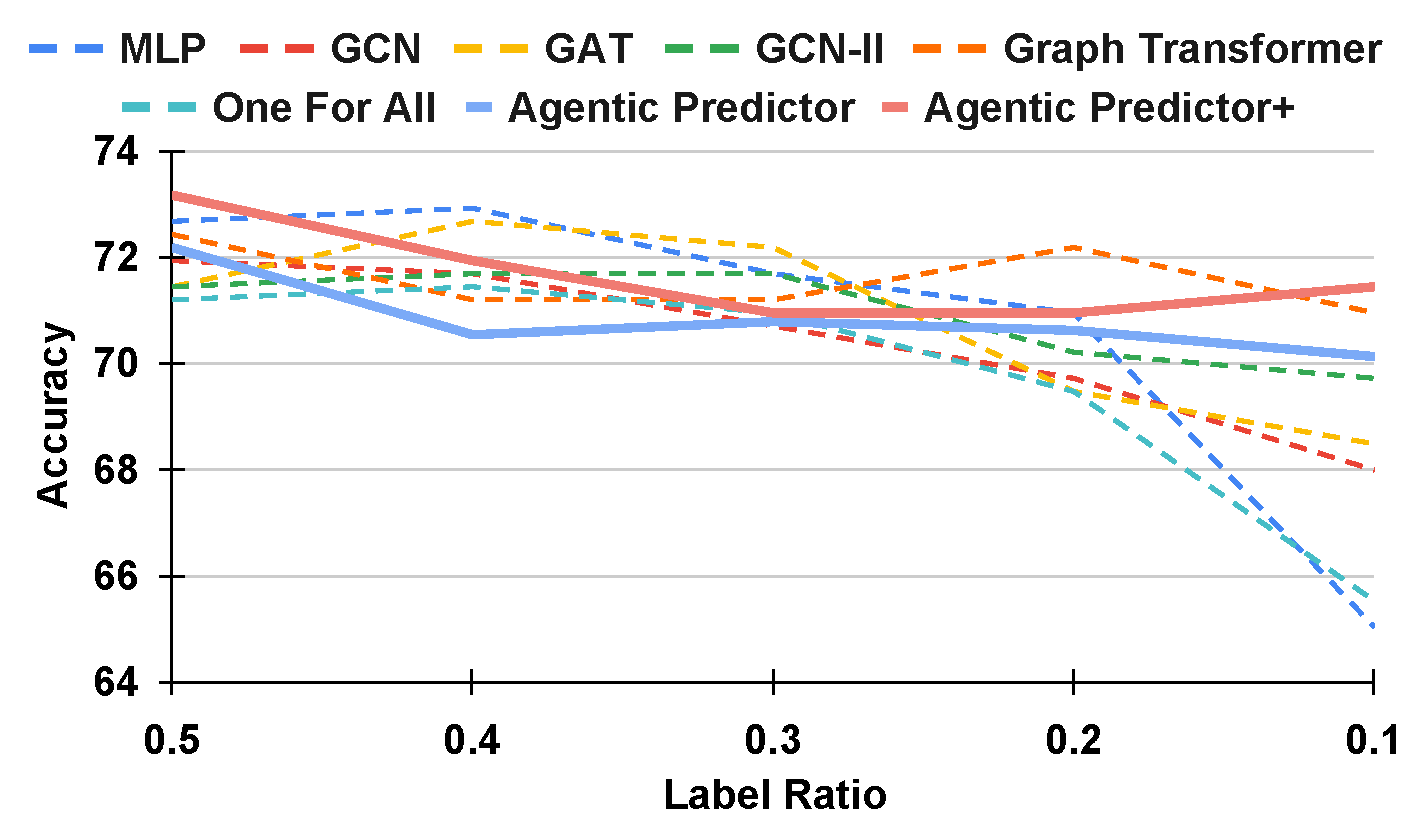
\includegraphics[width=0.24\textwidth]{figures/label_ratio_math_acc.pdf}%
        \label{figure:label_ratio_math_accuracy}
    }    
    \subfloat[Reasoning Tasks.]{
        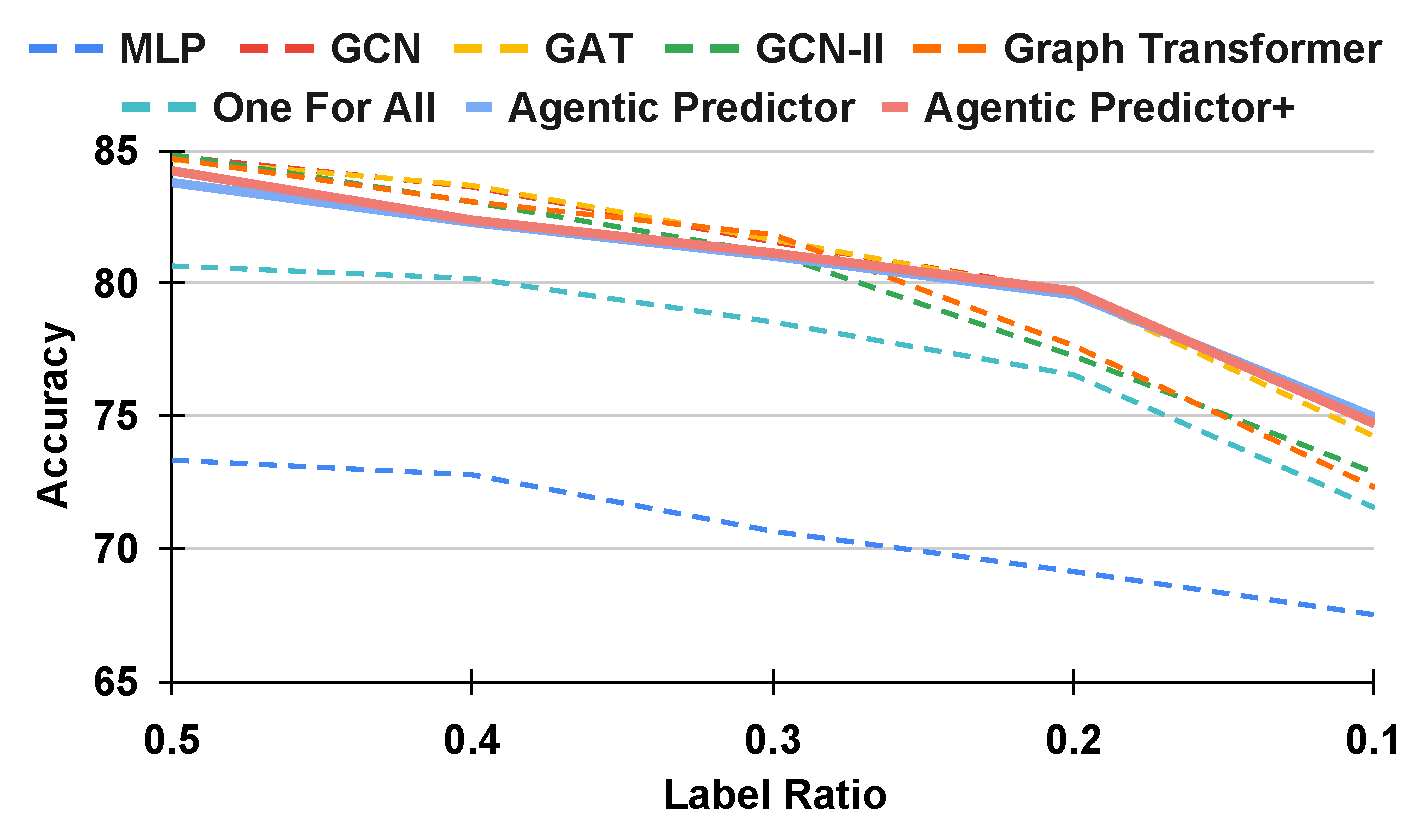
\includegraphics[width=0.24\textwidth]{figures/label_ratio_reason_acc.pdf}%
        \label{figure:label_ratio_reason_accuracy}
    }
    \subfloat[Average.]{
        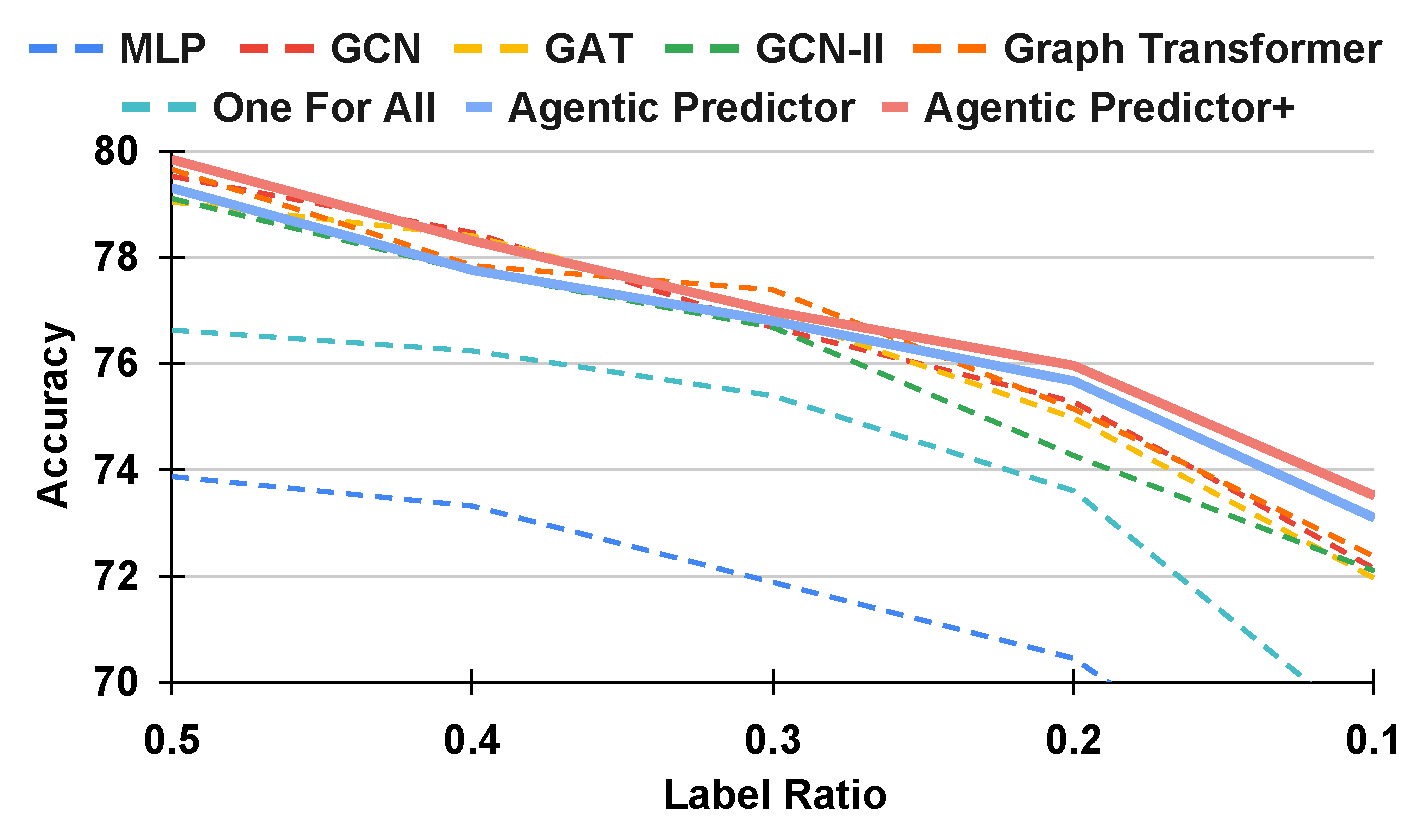
\includegraphics[width=0.24\textwidth]{figures/label_ratio_average_acc.pdf}%
        \label{figure:label_ratio_average_accuracy}
    }
    \hfil
    \subfloat[Code Generation.]{
            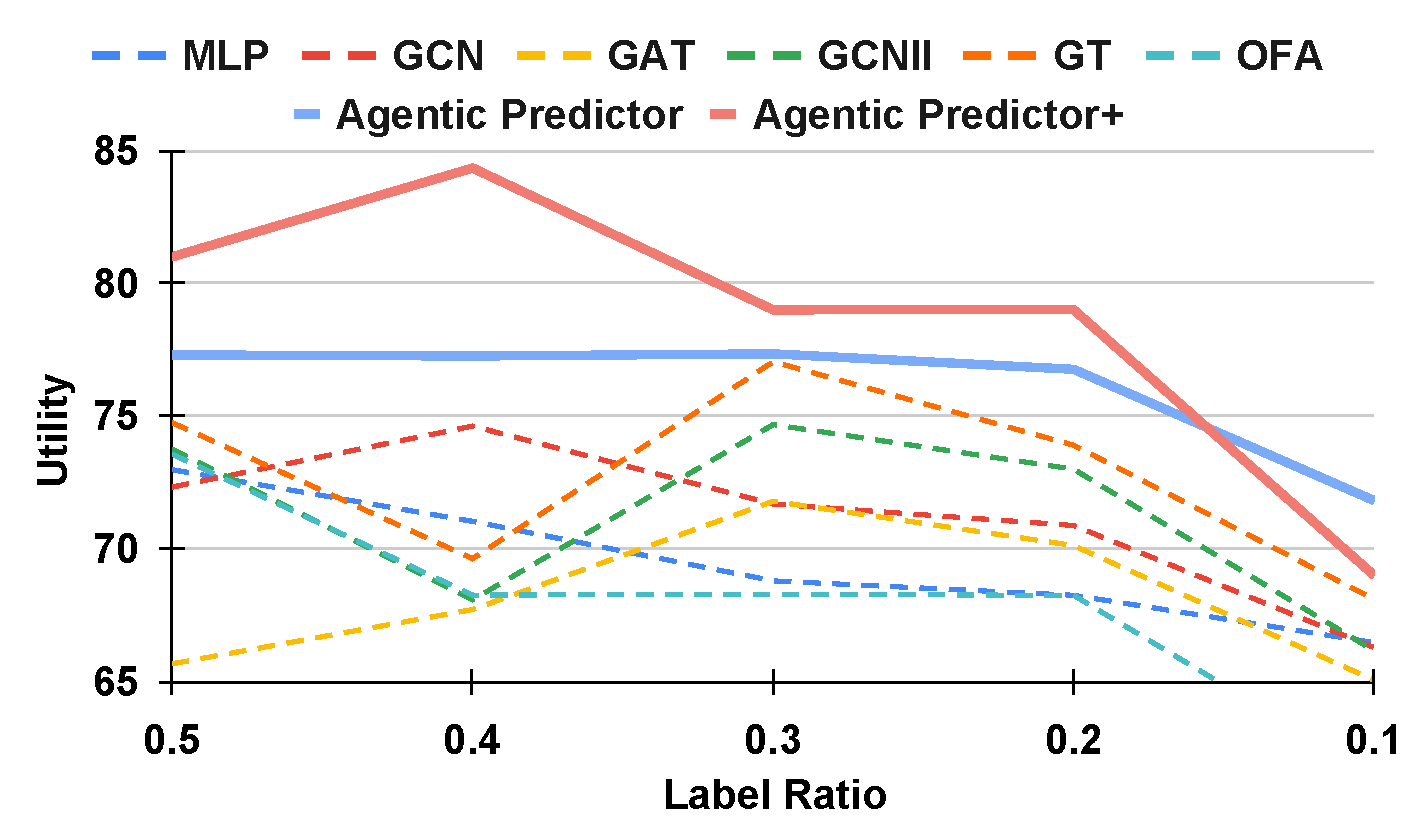
\includegraphics[width=0.24\textwidth]{figures/label_ratio_coding_uti.pdf}%
        \label{figure:label_ratio_coding_utility}
    }
    \subfloat[Math Problem.]{
        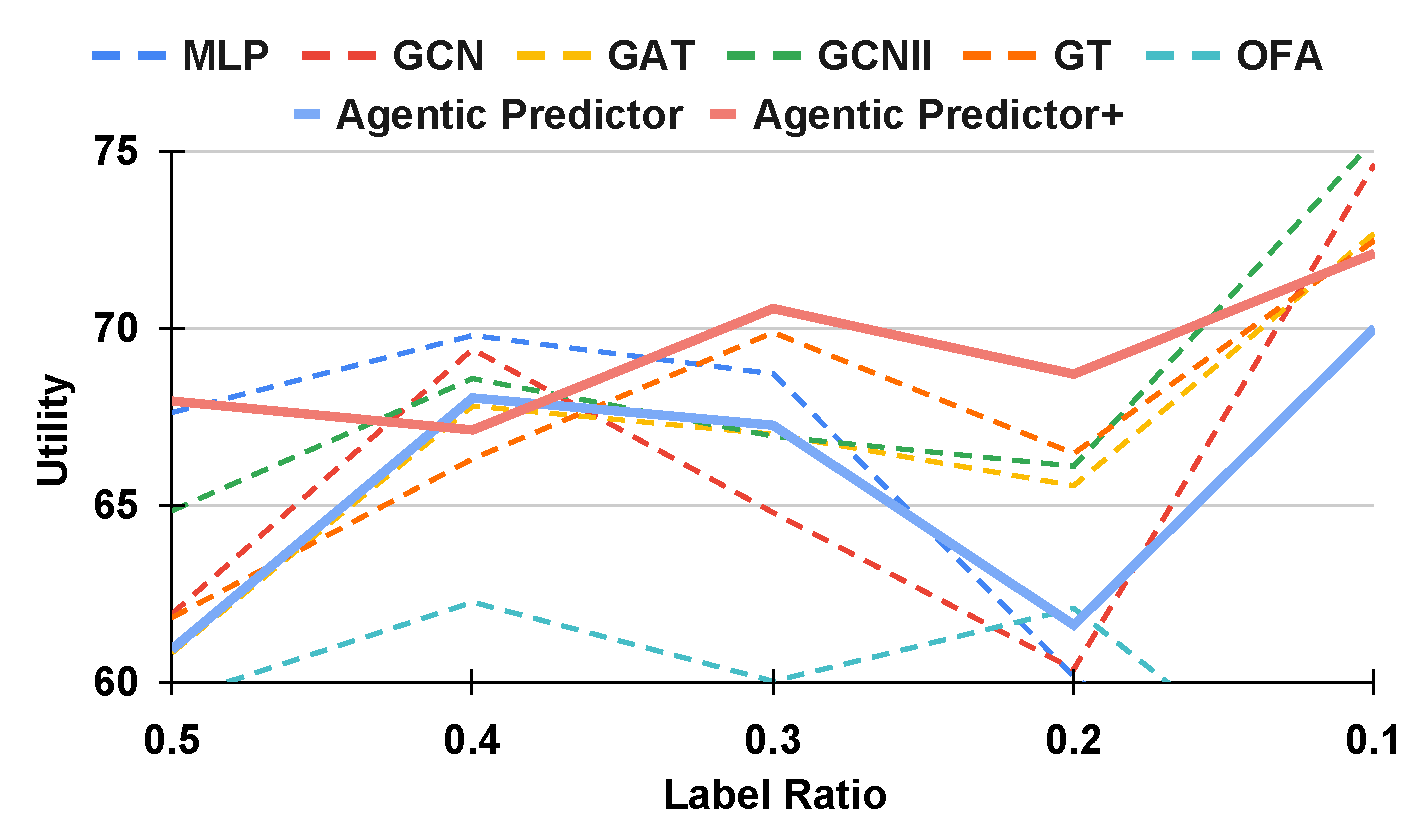
\includegraphics[width=0.24\textwidth]{figures/label_ratio_math_uti.pdf}%
        \label{figure:label_ratio_math_utility}
    }    
    \subfloat[Reasoning Tasks.]{
        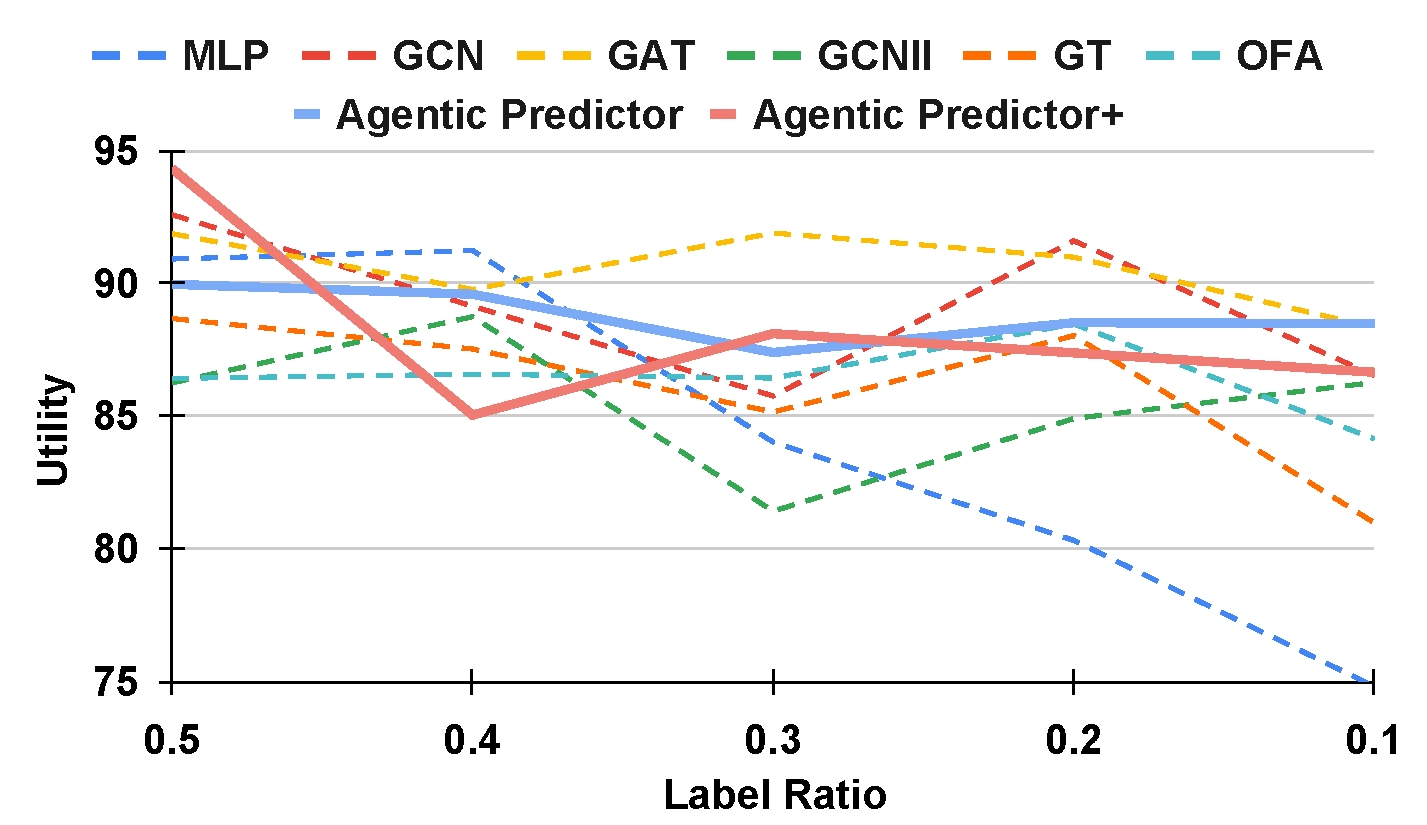
\includegraphics[width=0.24\textwidth]{figures/label_ratio_reason_uti.pdf}%
        \label{figure:label_ratio_reason_utility}
    }
    \subfloat[Average.]{
        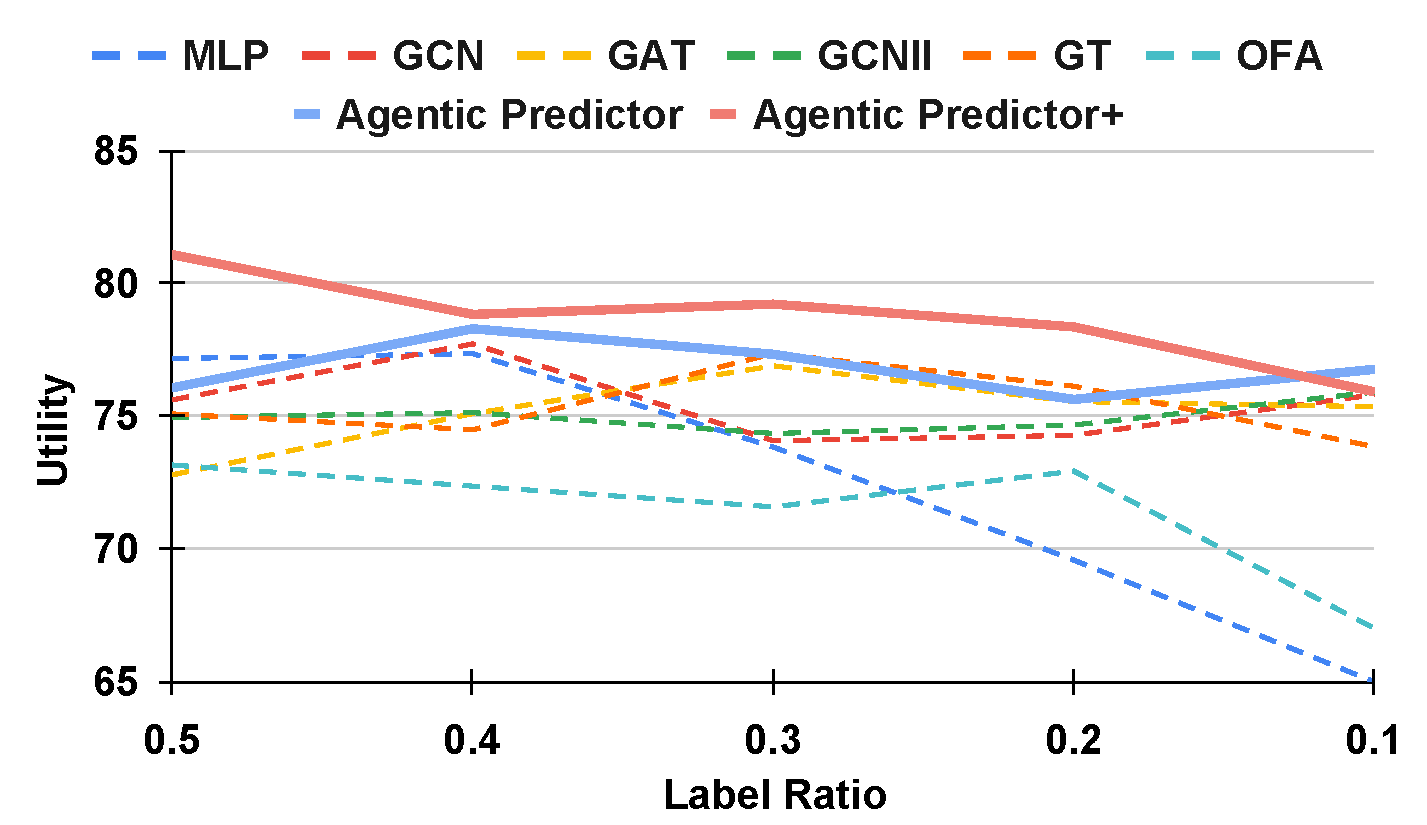
\includegraphics[width=0.24\textwidth]{figures/label_ratio_average_uti.pdf}%
        \label{figure:label_ratio_average_utility}
    }    
    
    \caption{Comparison of accuracy (upper) and utility (lower) between \ours{} and the baselines across varying label ratios.}
    \label{figure:label_ratio_full_results}
\vspace*{-0.4cm}
\end{figure}



% Whether using GNNs as predictors benefits the optimization of the agentic workflow?
\subsection{Workflow Optimization Results} \label{section:workflow_results}
In the main experiments, we demonstrate the feasibility and robustness of predicting agentic workflow performance. However, it remains an open question whether such predictions can effectively contribute to improving efficiency and to what extent they may introduce performance degradation in agentic workflows. To investigate this, we evaluate \emph{whether using \ours{} as a predictor enhances the optimization of agentic workflows compared to alternative baselines}. Specifically, we measure the performance improvement (or loss) incurred when using performance predictors.

To ensure a fair comparison, we adopt the same experimental setup as \citet{FLORA_Bench_25}, which provides a unified platform for optimizing agentic workflows and evaluating their performance. During the optimization process on each benchmark, a predictor is used to estimate the performance of candidate agentic workflows. These predicted performance values are treated as rewards to guide the optimization. Upon completion of the optimization, the quality of the resulting workflows is assessed based on their accuracy score on held-out test tasks.

We compare \ours{} against four baselines: (1) the \textbf{ground truth} baseline, which directly evaluates agentic workflows to obtain ground-truth performance scores (as done in the original AFlow\,\citep{AFlow_ICLR_25}); (2) two strong GNN-based predictors \textbf{GCN} and \textbf{GAT}; and (3) a \textbf{random} baseline, which assigns random performance scores as rewards. This experiment is conducted across five benchmarks: MATH, GSM8K, MBPP, HumanEval, and MMLU.

As in \autoref{table:workflow_optimization}, \ours{} consistently outperforms the random, GCN, and GAT baselines, achieving an average accuracy score of \textbf{74.43\%}, significantly higher than random (62.56\%), GCN (68.42\%), and GAT (71.00\%). Notably, as a predictor incurs zero search cost compared to the ground-truth's cost of \$39.83, this result underscores the effectiveness and efficiency of \ours{} as a reliable predictor for optimizing agentic workflows. Note that the search cost is $0$ because the predictors do not incur any LLM inference cost. Note that the search cost when using the performance predictor is effectively zero because the predictor incurs no LLM inference calls\,(i.e., no downstream task executions of task queries) to decide whether the current workflow has failed. The lightweight LLM update applied after each pass/fail decision, whose cost is about $0.005-0.01$ per update round with GPT-4.1-mini on the existing workflow, is \emph{excluded} from the reported costs for all methods.

In real-world deployments, \ours{} can be combined with any workflow generator\,(e.g., AFlow). In such cases, the overall cost decomposes into (1) the candidate-generation LLM cost (\emph{shared across all search strategies}) and (2) the evaluation cost. Our predictor reduces (2) by replacing most candidate evaluations with cheap, yet more accurate predictions, while incurring only a one-time training cost (see \S\ref{section:cost_analysis}). This analysis applies equally to the other predictors as well.



\begin{table}[t]
\caption{Workflow optimization performance based on the selected workflow across methods.}
\label{table:workflow_optimization}
\resizebox{\textwidth}{!}{%
\begin{tabular}{@{}c|cc|cc|ccc|cc@{}}
\toprule
\multirow{2}{*}{\textbf{Methods}} & \multicolumn{2}{c}{\textbf{Math Problems}} & \multicolumn{2}{|c}{\textbf{Code Generation}} & \multicolumn{3}{|c}{\textbf{Reasoning}} & \multicolumn{2}{|c}{\textbf{Average}} \\ \cmidrule(l){2-10} 
                                  & \textbf{MATH}            & \textbf{GSM8K}           & \textbf{MBPP}           & \textbf{HumanEval}          & \textbf{MMLU}    & \textbf{DROP}    & \textbf{HotpotQA}  & \textbf{Score}   & \textbf{Search Cost (\$)}  \\ \midrule \midrule
Ground Truth (AFlow)              & 87.38           & 94.53           & 73.22          & 97.20              & 83.10   & 84.25   & 69.94     & 84.23   & 39.83             \\ \midrule
Random                            & 78.40           & 75.23           & 67.84          & 76.34              & 42.87   & 80.42   & 16.86     & 62.56   & 0.00              \\
GCN                               & 79.22           & 86.16           & 68.23          & 97.46              & 46.43   & 82.33   & 19.14     & 68.42   & 0.00              \\
GAT                               & 80.11           & 86.22           & \textbf{68.62}          & 97.71              & 57.00   & 85.83   & \textbf{21.47}     & 71.00   & 0.00              \\ \midrule
\emph{\ours{}}          & \textbf{81.89}           & \textbf{92.65}           & 68.42          & \textbf{98.73}              & \textbf{79.70}   & \textbf{86.25}   & 13.37     & \textbf{74.43}   & 0.00              \\ \bottomrule
\end{tabular}%
}
\end{table}


\subsection{Transferability}
Considering that the MMLU benchmark encompasses various reasoning tasks, we further investigate the transferability of predictors trained on MMLU datasets to determine whether they can be used to optimize similar reasoning tasks, specifically DROP~\citep{DROP} and HotpotQA~\citep{HotpotQA}. As reported in \autoref{table:workflow_optimization}, the workflow optimized using \ours{} achieves competitive performance on these tasks: 86.25\% on DROP and 13.37\% on HotpotQA, demonstrating notable transferability. While performance on HotpotQA is lower than the baselines, the results remain broadly comparable, indicating that the workflows optimized via \ours{} maintain substantial effectiveness when transferred to closely related reasoning tasks. This highlights the practical potential of \ours{} for broader applicability in workflow optimization scenarios.

\section{Case Study} \label{section:case_study}
This section presents qualitative results from the workflow optimization process using \ours{} as the reward function across three domains.

\subsection{Code Generation} 
The code generation workflow on the HumanEval dataset demonstrates that the initial solution generation step often required subsequent refinement through explicit review and revision cycles. By systematically reviewing the initially generated code, and conditionally revising based on feedback from automated tests, the workflow substantially improved the final solution's correctness. This iterative approach effectively balanced computational cost and performance, resulting in solutions that were consistently more robust and accurate compared to single-step generations.
\begin{promptBox}{Workflow for Code Generation (HumanEval)} 
\begin{lstlisting}[language=Python]
from typing import Literal
import workspace.HumanEval.workflows.template.operator as operator
import workspace.HumanEval.workflows.round_19.prompt as prompt_custom
from metagpt.provider.llm_provider_registry import create_llm_instance
from metagpt.utils.cost_manager import CostManager

DatasetType = Literal["HumanEval", "MBPP", "GSM8K", "MATH", "HotpotQA", "DROP", "MMLU"]

class Workflow:
    def __init__(
        self,
        name: str,
        llm_config,
        dataset: DatasetType,
    ) -> None:
        self.name = name
        self.dataset = dataset
        self.llm = create_llm_instance(llm_config)
        self.llm.cost_manager = CostManager()
        self.custom = operator.Custom(self.llm)
        self.custom_code_generate = operator.CustomCodeGenerate(self.llm)
        self.test = operator.Test(self.llm)

    async def __call__(self, problem: str, entry_point: str):
        """
        Implementation of the workflow
        1. Generate initial solution using custom_code_generate.
        2. Review the solution using custom operator.
        3. Test the solution; if test fails, revise using custom operator and retest.
        """
        # Step 1: Generate initial solution
        initial_solution = await self.custom_code_generate(problem=problem, entry_point=entry_point, instruction="")

        # Step 2: Review the solution to improve quality
        reviewed = await self.custom(input=initial_solution['response'], instruction=prompt_custom.REVIEW_PROMPT)

        # Step 3: Test the reviewed solution
        test_result = await self.test(problem=problem, solution=reviewed['response'], entry_point=entry_point)

        # If test fails, revise solution based on test feedback and retest once
        if not test_result['result']:
            revised = await self.custom(input=reviewed['response'] + "\n" + test_result['solution'], instruction=prompt_custom.REVISE_PROMPT)
            test_result = await self.test(problem=problem, solution=revised['response'], entry_point=entry_point)
            final_solution = revised['response'] if test_result['result'] else reviewed['response']
        else:
            final_solution = reviewed['response']

        return final_solution, self.llm.cost_manager.total_cost
\end{lstlisting}
\end{promptBox}

\subsection{Math Problem}
In addressing mathematical problems using the MATH dataset, the workflow leverages an ensemble strategy by producing multiple candidate solutions, subsequently selecting the most consistent one via a self-consistency ensemble step. The selected solution was then further refined through an additional review process. This combined ensemble and review mechanism significantly enhanced solution quality, highlighting the value of ensemble techniques in solving complex mathematical reasoning tasks, while maintaining a controlled computational budget.
\begin{promptBox}{Workflow for Math Problem (MATH)} 
\begin{lstlisting}[language=Python]
from typing import Literal
import workspace.MATH.workflows.template.operator as operator
import workspace.MATH.workflows.round_88.prompt as prompt_custom
from metagpt.provider.llm_provider_registry import create_llm_instance
from metagpt.utils.cost_manager import CostManager

DatasetType = Literal["HumanEval", "MBPP", "GSM8K", "MATH", "HotpotQA", "DROP", "MMLU"]

class Workflow:
    def __init__(
        self,
        name: str,
        llm_config,
        dataset: DatasetType,
    ) -> None:
        self.name = name
        self.dataset = dataset
        self.llm = create_llm_instance(llm_config)
        self.llm.cost_manager = CostManager()
        self.custom = operator.Custom(self.llm)
        self.sc_ensemble = operator.ScEnsemble(self.llm)

    async def __call__(self, problem: str):
        """
        Implementation of the workflow with ensemble and review step
        """
        # Generate multiple candidate solutions using custom operator with different instructions
        candidates = []
        for i in range(3):
            response = await self.custom(input=problem, instruction=prompt_custom.SOLVE_PROMPT + f" Attempt {i+1}.")
            candidates.append(response['response'])

        # Use self-consistency ensemble to select the best solution
        ensemble_result = await self.sc_ensemble(solutions=candidates, problem=problem)
        best_solution = ensemble_result['response']

        # Review and refine the best solution
        review_response = await self.custom(input=problem + "\nSolution to review:\n" + best_solution, instruction=prompt_custom.REVIEW_PROMPT)
        final_solution = review_response['response']

        return final_solution, self.llm.cost_manager.total_cost
\end{lstlisting}
\end{promptBox}

\subsection{Reasoning Task}
For reasoning tasks on the MMLU dataset, the workflow combines multiple generation techniques, including custom-generated solutions with varying prompts and answers produced by specialized answer-generation operators, to diversify initial candidate answers. The self-consistency ensemble step effectively selected the most consistent candidate, which was subsequently subjected to rigorous review and format verification steps. This meticulous process, which included conditional regeneration and revision to ensure strict adherence to specified answer formats, proved highly effective in enhancing both accuracy and reliability of the final responses.
\begin{promptBox}{Workflow for Reasoning Task (MMLU)} 
\begin{lstlisting}[language=Python]
from typing import Literal
import workspace.MMLU.workflows.template.operator as operator
import workspace.MMLU.workflows.round_19.prompt as prompt_custom
from metagpt.provider.llm_provider_registry import create_llm_instance
from metagpt.utils.cost_manager import CostManager

DatasetType = Literal["HumanEval", "MBPP", "GSM8K", "MATH", "HotpotQA", "DROP", "MMLU"]

class Workflow:
    def __init__(
        self,
        name: str,
        llm_config,
        dataset: DatasetType,
    ) -> None:
        self.name = name
        self.dataset = dataset
        self.llm = create_llm_instance(llm_config)
        self.llm.cost_manager = CostManager()
        self.custom = operator.Custom(self.llm)
        self.answer_generate = operator.AnswerGenerate(self.llm)
        self.sc_ensemble = operator.ScEnsemble(self.llm)

    async def __call__(self, problem: str):
        """
        Implementation of the workflow with multiple custom answers, multiple AnswerGenerate answers, ensemble, review, and revision
        """
        # Step 1: Generate multiple candidate answers using custom operator with a concise prompt
        custom_answers = []
        for _ in range(2):
            custom_response = await self.custom(input=problem, instruction=prompt_custom.CUSTOM_PROMPT)
            custom_answer = custom_response['response']
            custom_answers.append(custom_answer)
        # Add 1 answer with diversity prompt to increase answer variety
        custom_diverse_response = await self.custom(input=problem, instruction=prompt_custom.CUSTOM_DIVERSE_PROMPT)
        custom_answers.append(custom_diverse_response['response'])

        # Step 2: Generate multiple candidate answers using AnswerGenerate operator to increase diversity
        answergen_answers = []
        for _ in range(2):
            answergen_response = await self.answer_generate(input=problem)
            answergen_answer = answergen_response['answer']
            answergen_answers.append(answergen_answer)

        # Step 3: Ensemble all candidate answers to select the most consistent answer
        all_answers = custom_answers + answergen_answers
        ensemble_response = await self.sc_ensemble(solutions=all_answers)
        ensemble_answer = ensemble_response['response']

        # Step 4: Review the ensemble answer to ensure format and correctness
        review_input = problem + "\nAnswer: " + ensemble_answer
        review_response = await self.custom(input=review_input, instruction=prompt_custom.REVIEW_PROMPT)
        reviewed_answer = review_response['response']

        # Step 5: If reviewed answer is not in correct format, regenerate with a stricter prompt
        if not reviewed_answer.startswith("Answer: Option "):
            strict_regen_input = problem + "\nPlease provide the final answer strictly in the format 'Answer: Option X'."
            strict_regen_response = await self.custom(input=strict_regen_input, instruction=prompt_custom.STRICT_REGEN_PROMPT)
            reviewed_answer = strict_regen_response['response']

        # Step 6: Revision step to refine the reviewed answer for strict format adherence
        revision_input = problem + "\nAnswer: " + reviewed_answer
        revision_response = await self.custom(input=revision_input, instruction=prompt_custom.REVISION_PROMPT)
        final_answer = revision_response['response']

        return final_answer, self.llm.cost_manager.total_cost
\end{lstlisting}
\end{promptBox}


% \section{Broader Impacts} \label{section:broader_impacts}
% The development of \ours{} has the potential to significantly reduce the computational and financial cost associated with optimizing LLM-based agentic workflows. By enabling efficient prediction of agent performance using multi-view representations and unsupervised pretraining, the method facilitates more scalable and accessible agentic system design across diverse domains. However, as with any predictive framework, there are possible societal risks. Misuse of the predictor could enable the rapid deployment of agentic systems in high-stakes applications (e.g., legal or medical domains) without sufficient evaluation, potentially leading to incorrect outcomes or biased decisions. Furthermore, if applied in surveillance or decision-making systems, biased workflow configurations could be propagated more efficiently. To mitigate these risks, we recommend incorporating human-in-the-loop validation for high-impact deployments and emphasize that our method is most suitable for early-stage design exploration rather than final system certification.


\section{Use of Large Language Models}
In preparing this submission, we employed ChatGPT-5 strictly as a tool for language refinement, including polishing text, improving clarity, and correcting grammatical and typographical errors. Its role was limited to grammar correction, sentence restructuring, and rephrasing for readability. All model-generated content was thoroughly reviewed and revised by the human authors to ensure accuracy, originality, and adherence to research-integrity standards. The LLMs did not contribute to the core research ideas, experimental design, or any substantive intellectual components of the work. Note that LLMs also served as baselines for LLM-based prediction (\S\ref{section:llm_fewshot_results}) and case-study (\S\ref{section:case_study}) experiments, as described above.